% ---
% Capitulo de Referencial Teorico
% ---

\chapter{Referencial Teórico\label{cha:theory-framework}}

Este capítulo estabelece a base conceitual do trabalho. A Seção \ref{sec:density-clustering} descreve como o agrupamento baseado em densidade funciona e por que ele se reduz, em todas as suas variantes, ao cálculo de uma única árvore geradora mínima. A Seção \ref{sec:coresg-context} apresenta o \ac{CORE-SG} nesse contexto. A Seção \ref{sec:problems} formaliza os dois problemas que este trabalho ataca. A Seção \ref{sec:discarded} percorre as abordagens que foram consideradas e posteriormente descartadas ou substituídas, incluindo a mudança de metodologia ocorrida entre a qualificação e a versão final desta pesquisa. A Seção \ref{sec:adopted} justifica as decisões finalmente adotadas e descreve o princípio de funcionamento de cada uma. A Seção \ref{sec:related-work} situa o trabalho na literatura.

% =====================================================================
\section{Agrupamento baseado em densidade\label{sec:density-clustering}}
% =====================================================================

\subsection{O DBSCAN e a noção de conectividade por densidade\label{sec:dbscan}}

O \ac{DBSCAN} \cite{dbscan} formaliza a intuição de que um grupo é uma região onde os objetos se concentram, separada de outras regiões por áreas de baixa concentração. Ele opera com dois parâmetros. O primeiro, $\varepsilon$, é um raio, e define a vizinhança de um objeto como o conjunto de objetos a distância menor ou igual a $\varepsilon$ dele. O segundo, $\mpts$, é uma contagem mínima, e define quantos objetos precisam estar dentro dessa vizinhança para que o objeto central seja considerado denso.\\

Um objeto cuja vizinhança de raio $\varepsilon$ contém ao menos $\mpts$ objetos é chamado de objeto \textit{core}. Dois objetos \textit{core} pertencem ao mesmo grupo se existe uma cadeia de objetos \textit{core} ligando um ao outro em que cada elo está a distância no máximo $\varepsilon$ do seguinte. Objetos que não são \textit{core} e não estão na vizinhança de nenhum objeto \textit{core} são declarados ruído. Essa definição é o que confere ao método sua robustez a ruído e sua capacidade de detectar grupos de forma arbitrária: nada na construção presume convexidade, esfericidade ou tamanho comparável entre grupos.\\

A dificuldade prática do \ac{DBSCAN} é que o resultado depende fortemente de $\varepsilon$, e um único valor de $\varepsilon$ não é adequado quando os grupos do conjunto diferem em densidade. Um valor que isola corretamente os grupos densos funde os esparsos com o ruído; um valor que preserva os esparsos funde os densos entre si.\\

\subsection{O HDBSCAN* e a hierarquia de densidade\label{sec:hdbscan}}

O \ac{HDBSCAN*} \cite{hdbscan} resolve essa dificuldade eliminando $\varepsilon$ como parâmetro. Em vez de produzir o agrupamento correspondente a um único limiar, ele produz a hierarquia completa dos agrupamentos correspondentes a todos os limiares possíveis, deixando ao usuário a escolha de onde e como cortá-la. Dois conceitos sustentam essa construção.\\

O primeiro é a \textit{core distance}. Dado um conjunto de dados $X = \{x_1, \dots, x_n\}$ com $n$ objetos e uma medida de distância $d(\cdot,\cdot)$, a \textit{core distance} de um objeto $x \in X$ com relação a $\mpts$ é a distância de $x$ ao seu $\mpts$-ésimo vizinho mais próximo, incluindo o próprio $x$ na contagem:
\begin{equation}
\label{eq:coredist}
\coredist^{\mpts}(x) = d(x, \mathrm{NN}_{\mpts}(x)),
\end{equation}
onde $\mathrm{NN}_{\mpts}(x)$ denota o $\mpts$-ésimo vizinho mais próximo de $x$. Essa quantidade é pequena em regiões densas e grande em regiões esparsas, e é exatamente o menor valor de $\varepsilon$ para o qual $x$ seria considerado \textit{core}.\\

O segundo é a \textit{mutual reachability distance}, que substitui a distância original entre dois objetos por
\begin{equation}
\label{eq:mrd}
\mrd^{\mpts}(x,y) = \max \left\{ \coredist^{\mpts}(x),\; \coredist^{\mpts}(y),\; d(x,y) \right\},
\end{equation}
para $x, y \in X$. Essa transformação infla as distâncias em regiões esparsas, onde as \textit{core distances} são grandes, e deixa intactas as distâncias em regiões densas, onde a distância original domina. O valor de $\mrd^{\mpts}(x,y)$ é o menor $\varepsilon$ para o qual $x$ e $y$ estariam densamente conectados. Seu efeito prático é impedir que o agrupamento por ligação simples encadeie grupos distintos através de pontos de ruído situados entre eles.\\

Construir o grafo completo sobre $X$ ponderado por $\mrd^{\mpts}$ e extrair sua \ac{MST} produz uma árvore cujos pesos de aresta, ordenados de forma crescente, são exatamente as alturas de fusão do dendrograma de ligação simples nesse espaço transformado. A hierarquia do \ac{HDBSCAN*} é esse dendrograma, e cortá-lo em um limiar $\varepsilon$ recupera o agrupamento do \ac{DBSCAN} para aquele $\varepsilon$, em sua variante que trata ruído explicitamente \cite{hdbscan}. Tudo o que o método produz é, portanto, determinado por um único objeto, a $\mathrm{MST}_{\mpts}$, e pelo parâmetro que a define.\\

\subsection{A extração de agrupamentos planos\label{sec:fosc}}

Uma hierarquia não é, por si só, uma partição dos dados. Obter uma partição exige escolher onde cortá-la, e um corte horizontal único, em um limiar fixo de densidade, é incapaz de capturar a granularidade que a hierarquia representa, precisamente porque grupos de densidades diferentes se dissolvem em alturas diferentes. O \ac{FOSC} \cite{fosc} resolve isso realizando cortes locais em níveis distintos da hierarquia, selecionando o conjunto de grupos que maximiza uma função objetivo. Na sua forma não supervisionada, essa função é a estabilidade do grupo, que pode ser interpretada como o intervalo de densidade ao longo do qual o grupo permanece coeso antes de se fragmentar ou se dissolver em ruído. Essa é a rotina de extração usada pelo \ac{HDBSCAN*} e é o que produz o agrupamento plano comparado nos experimentos deste trabalho.\\

\subsection{O arcabouço unificado e o papel do $\mpts$\label{sec:framework}}

Foi demonstrado que essa estrutura não é particular ao \ac{HDBSCAN*} \cite{framework-density-clustering}. Métodos baseados em densidade, supervisionados ou não, podem ser descritos como instâncias de um mesmo arcabouço, cuja operação central é o cálculo da \ac{MST} de um grafo completo em um espaço transformado por uma estimativa de densidade, parametrizada por $\mpts$. Agrupamento, detecção de anomalias, classificação semissupervisionada e regressão baseada em densidade diferem no que é extraído dessa árvore, não em como ela é obtida.\\

Isso confere ao $\mpts$ um papel especial. Ele é um fator de suavização: ao aumentar $\mpts$, mais vizinhos entram na estimativa de densidade, as \textit{core distances} crescem, e a paisagem de densidade se torna mais suave, o que faz grupos pequenos ou pouco densos desaparecerem e grupos vizinhos se fundirem. Ao diminuir $\mpts$, a estimativa se torna mais sensível a variações locais, o que revela estrutura fina mas também torna o método mais suscetível a flutuações amostrais. Não existe procedimento principiado para escolher $\mpts$ antes de examinar os dados, e nenhum valor único é apropriado quando os grupos diferem em densidade. A consequência operacional é que é usual executar o método sobre uma faixa de valores de $\mpts$ e comparar as hierarquias resultantes.\\

Essa varredura é cara. A complexidade do \ac{HDBSCAN*} é dominada pelo cálculo da \ac{MST} sobre o grafo completo, que custa $O(n^2 d)$ para $n$ objetos de dimensionalidade $d$. Como cada valor de $\mpts$ define um conjunto diferente de \textit{core distances} e, portanto, um espaço transformado diferente, cada valor exige o seu próprio cálculo. Uma varredura sobre $t$ valores distintos de $\mpts$ custa $t$ vezes o custo de uma execução, o que se torna proibitivo justamente nos conjuntos grandes em que a análise exploratória é mais necessária.\\

% =====================================================================
\section{O CORE-SG\label{sec:coresg-context}}
% =====================================================================

\subsection{Construção\label{sec:coresg-construction}}

O \ac{CORE-SG} \cite{core-sg} elimina a repetição do custo quadrático ao observar que um único grafo pode servir a todos os valores de $\mpts$ de uma vez. Definindo $\kmax$ como o maior valor de interesse do parâmetro, o grafo é
\begin{equation}
\label{eq:coresg}
\mathrm{CORE\text{-}SG}_{\kmax} = \kmax\text{-}\mathrm{NNG} \;\cup\; \mathrm{MST}_{\kmax},
\end{equation}
isto é, a união do grafo de $\kmax$ vizinhos mais próximos com a \ac{MST} do grafo completo ponderado por $\mrd^{\kmax}$. Ambas as estruturas são subprodutos naturais de uma execução de um método baseado em densidade: as distâncias aos $k$ vizinhos de cada objeto já precisam ser calculadas para obter as \textit{core distances}, e a \ac{MST} é o produto final do método. Uma única execução, portanto, basta para construir o \ac{CORE-SG}.\\

O resultado é formalizado pelo seguinte teorema.\\

\textbf{Teorema 1} \cite{core-sg}\textbf{.} Seja $G_i$ o grafo completo sobre $X$ ponderado por $\mrd^{i}$, seja $M_i$ o conjunto de todas as \ac{MST}s de $G_i$, e seja $\mathrm{MST}_{\kmax}$ uma \ac{MST} qualquer de $G_{\kmax}$. Então
\[
\forall\, i < \kmax \;:\; \exists\, \mathrm{MST}_i \in M_i \;:\; \mathrm{MST}_i \subseteq \mathrm{MST}_{\kmax} \cup \kmax\text{-}\mathrm{NNG}.
\]
Em palavras, para todo valor do parâmetro abaixo de $\kmax$ existe pelo menos uma árvore geradora mínima do grafo completo correspondente que está inteiramente contida na união \eqref{eq:coresg}. O caso $i = \kmax$ é trivial, pois a própria $\mathrm{MST}_{\kmax}$ compõe a união.\\

Extrair a $\mathrm{MST}_{\mpts}$ para um $\mpts$ específico se reduz, então, a repesar as $O(n\kmax)$ arestas armazenadas com $\mrd^{\mpts}$ e executar um algoritmo de árvore geradora mínima sobre essa lista, o que é linear no número de arestas a menos de um fator logarítmico. O grafo resultante é significativamente mais esparso que o completo, com crescimento linear em $n$ quando $\kmax \ll n$, e é compatível com qualquer espaço métrico, isto é, não impõe restrições sobre a representação dos dados ou sobre a medida de distância utilizada.\\

\subsection{Por que a união basta\label{sec:coresg-why}}

A justificativa do Teorema 1 decorre diretamente do comportamento da \textit{mutual reachability distance} sob variação de $\mpts$. Conforme $\mpts$ aumenta, a \textit{core distance} de cada objeto tende a aumentar, pois abrange mais vizinhos, enquanto a distância métrica permanece constante, por não depender do parâmetro. Enquanto a distância métrica se mantiver maior que ambas as \textit{core distances}, a \textit{mutual reachability distance} permanece igual a ela. Em resumo, com o aumento de $\mpts$, o peso de uma aresta tende a permanecer ou a crescer, nunca a diminuir.\\

Considere uma aresta $(p,q)$ pertencente a alguma $\mathrm{MST}_{\mpts}$ com $\mpts \leq \kmax$. Ela deve ser uma das arestas de menor peso que conectam duas partições do conjunto de dados. Se $(p,q) \in \mathrm{MST}_{\kmax}$, ela já faz parte da união em \eqref{eq:coresg}. Caso contrário, deve existir outra aresta $(r,s) \in \mathrm{MST}_{\kmax}$ conectando as mesmas partições, cujo peso é, pelas propriedades da \ac{MST}, no máximo igual ao de $(p,q)$. Restam dois casos. Se o peso de $(p,q)$ é determinado por uma \textit{core distance}, digamos $\mrd^{\mpts}(p,q) = \coredist^{\mpts}(p)$, então $d(p,q) \leq \coredist^{\mpts}(p)$, ou seja, $q$ está entre os $\mpts$ vizinhos mais próximos de $p$; a aresta pertence então ao grafo de $\mpts$ vizinhos mais próximos, que está contido no de $\kmax$ vizinhos porque $\mpts \leq \kmax$. Se o peso é determinado pela distância métrica, $(r,s)$ pode substituir $(p,q)$ sem alterar o resultado, pois liga as mesmas partições com peso não maior.\\

Essa análise expõe uma assimetria entre os dois grafos constituintes que este trabalho explora. Pela definição \eqref{eq:mrd}, o peso de uma aresta cai em um de dois casos. Quando $d(x,y)$ é pequena em relação às duas \textit{core distances}, o peso é determinado pelas \textit{core distances} sozinhas, que são recuperáveis do \ac{k-NNG}. As arestas que carregam informação ainda não presente são aquelas em que a distância entre os pontos domina ambas as \textit{core distances}, ou seja, arestas longas que ligam componentes que a vizinhança não alcança. É a $\mathrm{MST}_{\kmax}$ que as fornece. A Figura \ref{fig:coresg-edge-case} ilustra um caso em que o \ac{k-NNG} sozinho não contém todas as arestas da \ac{MST}, o que estabelece que o segundo termo da união é necessário, e a união das duas estruturas garante a conectividade global.\\

\begin{figure}[htb!]
\centering
\caption{\label{fig:coresg-edge-case} Exemplo de um \ac{k-NNG} em (a) que não contém a \ac{MST} em (b) para um grafo completo $G_{\mpts}$, onde $k=\mpts=4$.}
\includegraphics[width=\textwidth]{cap_materias_e_metodos/coresg_edge_case.eps}
Fonte: Recriação autoral do original \cite{core-sg}.
\end{figure}

Há um segundo caso, mais sutil, em que o \ac{k-NNG} sozinho é insuficiente, e ele não envolve desconexão alguma. Dois pontos podem estar próximos no espaço e, ainda assim, ausentes das listas de vizinhos um do outro, se cada um deles estiver dentro de uma região densa cujos $k$ vizinhos mais próximos são todos internos a ela. Nessa situação, o grafo completo oferece uma aresta curta ligando as duas regiões diretamente, enquanto o \ac{k-NNG} só as liga por um percurso que contorna toda a estrutura. É a configuração em ferradura ilustrada pelo trabalho original do \ac{CORE-SG} \cite{core-sg} e reproduzida na Figura \ref{fig:horseshoe}: os dois grafos são conexos, mas a árvore geradora extraída de cada um difere, porque a do grafo completo pode usar a corda curta e descartar a aresta mais pesada do arco, e a extraída do \ac{k-NNG} não pode.\\

\begin{figure}[htb!]
\centering
\caption{\label{fig:horseshoe} A configuração em ferradura. As regiões densas $A$ e $B$ estão próximas no espaço, mas os $k$ vizinhos mais próximos de cada ponto de $A$ estão todos dentro de $A$, de modo que a corda $A$--$B$ não pertence ao \ac{k-NNG}. Os dois grafos são conexos. A árvore geradora do grafo completo usa a corda de peso 0,76 e descarta a aresta de peso 1,16 do arco; a árvore extraída do \ac{k-NNG} é obrigada a manter essa aresta, o que altera a altura de fusão correspondente na hierarquia.}
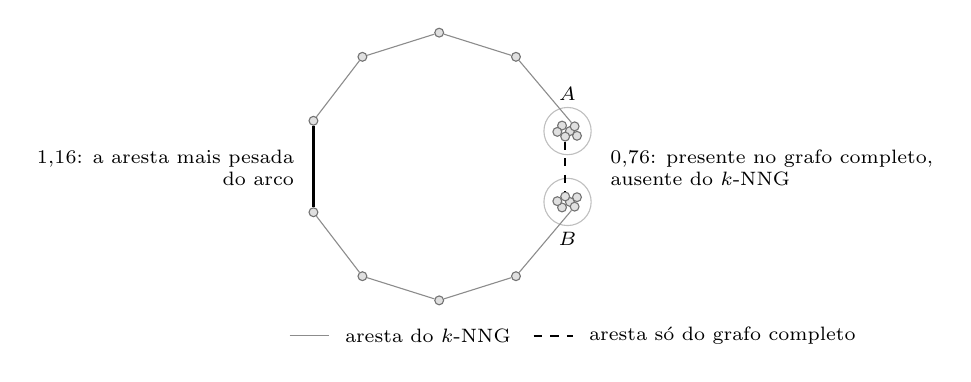
\begin{tikzpicture}[
  pt/.style={circle, draw=black!55, fill=black!12, inner sep=0pt, minimum size=3.2pt},
  knn/.style={black!45, thin},
  heavy/.style={black, thick},
  chord/.style={black, thick, dashed},
  lb/.style={font=\scriptsize}
]
% ---- regiao densa A
\draw[black!25] (1.63,0.45) circle (0.30);
\foreach \x/\y in {1.56/0.52, 1.75/0.39, 1.66/0.45, 1.50/0.44}
  \node[pt] at (\x,\y) {};
\node[pt] (A1) at (1.60,0.38) {};
\node[pt] (A2) at (1.72,0.51) {};
\node[lb] at (1.63,0.92) {$A$};
% ---- regiao densa B
\draw[black!25] (1.63,-0.45) circle (0.30);
\foreach \x/\y in {1.56/-0.52, 1.75/-0.39, 1.66/-0.45, 1.50/-0.44}
  \node[pt] at (\x,\y) {};
\node[pt] (B1) at (1.60,-0.38) {};
\node[pt] (B2) at (1.72,-0.51) {};
\node[lb] at (1.63,-0.92) {$B$};
% ---- arco esparso
\node[pt] (s1) at ( 0.975, 1.393) {};
\node[pt] (s2) at ( 0.000, 1.700) {};
\node[pt] (s3) at (-0.975, 1.393) {};
\node[pt] (s4) at (-1.597, 0.581) {};
\node[pt] (s5) at (-1.597,-0.581) {};
\node[pt] (s6) at (-0.975,-1.393) {};
\node[pt] (s7) at ( 0.000,-1.700) {};
\node[pt] (s8) at ( 0.975,-1.393) {};
\draw[knn] (A2) -- (s1);
\draw[knn] (s1) -- (s2) -- (s3) -- (s4);
\draw[heavy] (s4) -- (s5);
\draw[knn] (s5) -- (s6) -- (s7) -- (s8);
\draw[knn] (s8) -- (B2);
% ---- corda
\draw[chord] (A1) -- (B1);
\node[lb, anchor=west] at (2.05, 0.10) {$0{,}76$: presente no grafo completo,};
\node[lb, anchor=west] at (2.05,-0.15) {ausente do $k$-NNG};
\node[lb, anchor=east] at (-1.72, 0.10) {$1{,}16$: a aresta mais pesada};
\node[lb, anchor=east] at (-1.72,-0.15) {do arco};
% ---- legenda
\draw[knn]   (-1.90,-2.15) -- (-1.40,-2.15);
\node[lb, anchor=west] at (-1.32,-2.15) {aresta do $k$-NNG};
\draw[chord] ( 1.20,-2.15) -- ( 1.70,-2.15);
\node[lb, anchor=west] at ( 1.78,-2.15) {aresta só do grafo completo};
\end{tikzpicture}\\
Fonte: Autoral, sobre a configuração descrita em \cite{core-sg}.
\end{figure}

Esse segundo caso é o que torna a questão empírica em vez de teórica: saber que o \ac{k-NNG} é conexo não basta para concluir que a árvore geradora é dispensável. A Seção \ref{sec:res-connectivity} mede quanto esse resíduo custa em dados reais.\\

% =====================================================================
\section{O problema atacado\label{sec:problems}}
% =====================================================================

\subsection{A construção centralizada e o limite de memória\label{sec:problem-scale}}

O \ac{CORE-SG} resolve o custo de repetir a análise sobre vários valores de $\mpts$, mas sua construção segue um modelo de execução centralizado. Os dois grafos constituintes são calculados e armazenados em um único espaço de memória, sobre o conjunto de dados inteiro, de uma só vez. A \ac{MST} que compõe a segunda metade é, em particular, definida sobre um grafo completo, o que impede que sua construção seja distribuída sem que se materialize ou se percorra $O(n^2)$ pares.\\

Em aceleradores gráficos, essa característica deixa de ser uma questão de tempo e passa a ser uma questão de viabilidade. Há uma assimetria entre os dois recursos que um acelerador oferece. Poder de cálculo é elástico: se a máquina é lenta, espera-se mais, e o resultado eventualmente sai. Memória de dispositivo não é elástica: se a estrutura não cabe, nenhuma quantidade de tempo resolve. A memória de uma \ac{GPU} é tipicamente uma ou duas ordens de grandeza menor que a memória principal de um servidor, é a única memória a que os núcleos do dispositivo têm acesso direto, e essa diferença não tem acompanhado o crescimento do poder de cálculo das próprias \ac{GPU}s.\\

A consequência é um teto abrupto. Uma construção de instância única com $d = 128$ e $\kmax = 32$ ocupa 944 bytes por ponto no dispositivo, o que coloca o limite em torno de $9{,}1 \times 10^6$ pontos em um acelerador de 8 GB. Abaixo desse teto, a construção é rápida; acima dele, ela não executa.\\

O aspecto decisivo é que acrescentar aceleradores ao sistema não move esse teto. Uma construção monolítica não é dividida entre dispositivos: um segundo acelerador não contribui com sua memória, apenas permanece ocioso. O conjunto de dados que não cabe em uma \ac{GPU} continua não cabendo em quatro. Distribuir a construção entre dispositivos só resolve o problema se o método for decomposto de forma que o estado por dispositivo não cresça com o tamanho do conjunto, o que é uma propriedade do projeto do algoritmo e não do hardware.\\

\subsection{Localidade e decomponibilidade\label{sec:incremental-framework}}

A teoria de computação sobre grafos fornece o vocabulário para analisar quando uma estrutura admite esse tipo de decomposição \cite{incremental-computations}. Um problema é dito \textit{limitado} se o custo de atualizá-lo é polinomial nas taxas de mudança da entrada e da saída, o que garante que o custo não dependa do tamanho do grafo. Está demonstrado que consultas fundamentais em grafos são \textit{ilimitadas}, o que impede que computações sobre elas estejam sob esse limite.\\

O mesmo trabalho, entretanto, introduz dois conceitos que conferem eficiência prática mesmo sob operações ilimitadas, e que se aplicam tanto à atualização de uma estrutura quanto à sua construção particionada. O primeiro é o de \textit{computação localizável}: problemas cuja resolução exige apenas a inspeção da vizinhança local de cada elemento, o que delimita o custo pelo tamanho dessa região. O segundo é o de \textit{limitação relativa}: o esforço é comparado ao de reexecutar o algoritmo completo, de modo que a computação se concentre apenas naquilo que de fato importa.\\

A localidade é a propriedade que governa a decomponibilidade. Uma estrutura cuja definição depende apenas de regiões pode ser construída por partes, desde que cada parte contenha a região de que depende; uma estrutura cuja definição é global não pode, porque nenhuma parte contém o que é necessário para decidir. Ambos os conceitos aparecem em algoritmos da literatura sobre grafos dinâmicos. O \ac{MoSSo} \cite{mosso} emprega um agrupamento grosseiro que organiza os vértices por similaridade através de uma variante de \ac{LSH}, reduzindo o espaço de busca de candidatos à fusão, e recorre ao \ac{MCMC} para amostrar uniformemente as vizinhanças dos vértices escolhidos, evitando explorá-las por completo. O \ac{DPGS} \cite{dpgs} também agrupa vértices por similaridade através de \ac{LSH}, sob a hipótese de que vértices próximos são mais propensos a minimizar sua função objetivo, baseada em \ac{MDL}. O IncBoost \cite{inc-boost}, por sua vez, identifica os vértices afetados por cada nova conexão, aplica a eles uma função de vértice e propaga essa aplicação aos vizinhos apenas quando necessário, mantendo uma fronteira de vértices a processar na iteração seguinte.\\

\subsection{A assimetria entre os dois grafos constituintes\label{sec:asymmetry}}

A observação que organiza todo este trabalho é que os dois grafos constituintes do \ac{CORE-SG} se comportam de maneira oposta sob essa taxonomia.\\

O \ac{k-NNG} é localizável. Sua construção depende exclusivamente das vizinhanças de cada vértice, de modo que a lista de vizinhos de um ponto é determinada pelos pontos geometricamente próximos a ele, e não pelo conjunto inteiro. A Figura \ref{fig:knng-increment-reaction} ilustra esse comportamento no caso de um ponto acrescentado a um grafo existente: alguns vértices em torno dele o integram à sua vizinhança, mesmo quando eles próprios não fazem parte da vizinhança do vértice novo, enquanto vértices mais distantes mantêm suas vizinhanças intactas. O \ac{k-NNG} encapsula as localidades do conjunto de dados, e isso é o que torna sua construção decomponível: um bloco de pontos contém, para a maioria de seus membros, boa parte da informação de que suas listas de vizinhança precisam.\\

\begin{figure}[htb!]
\centering
\caption{\label{fig:knng-increment-reaction} Comportamento do incremento no \ac{k-NNG}, arestas coincidentes foram representadas como uma só.}
\includegraphics[width=\textwidth]{cap_materias_e_metodos/knng_increment_reaction.eps}
Fonte: Autoral.
\end{figure}

A \ac{MST} não é localizável. Ela é uma estrutura inerentemente global: a decisão de incluir ou não uma aresta depende de quais partições do grafo ela conecta, e isso é uma propriedade de todo o grafo, não de uma região dele. Nenhum bloco de pontos contém a informação necessária para decidir quais de suas arestas pertencem à árvore do conjunto completo.\\

Há, além disso, um agravante específico ao \ac{CORE-SG} que não se aplica ao cálculo de \ac{MST}s em geral. A árvore de que se precisa não é a de um grafo esparso com pesos fixos, mas a de um grafo \textit{completo} cujos $O(n^2)$ pesos são todos função de $\mpts$, e portanto se deslocam quando o parâmetro muda. Calcular ou manter uma árvore sobre um grafo que nunca é materializado, e cujos pesos dependem de um parâmetro que o usuário varia livremente, é um problema substancialmente mais difícil que o problema clássico.\\

A Figura \ref{fig:knng-is-enough} ilustra a fronteira entre os dois casos. Se muitos vértices próximos entre si estiverem agrupados longe do restante do conjunto, as arestas do \ac{k-NNG} são insuficientes até mesmo para conectar os componentes, e uma aresta que alcance além da $k$-vizinhança é necessária. Em casos menos extremos, porém, os $k$ vizinhos mais próximos de um vértice, por serem os mais próximos, correspondem às arestas de menor peso incidentes a ele, que é exatamente o material de que uma \ac{MST} é feita.\\

\begin{figure}[htb!]
\centering
\caption{\label{fig:knng-is-enough} Como o \ac{k-NNG} pode auxiliar em estimar arestas para a \ac{MST}.}
\includegraphics[width=\textwidth]{cap_materias_e_metodos/knng_is_enough.eps}
Fonte: Autoral.
\end{figure}

Essa assimetria determina o desenho do método. O \ac{k-NNG}, por ser localizável, é decomposto; a \ac{MST}, por ser global, não é decomposta, mas substituída.\\

\subsection{O que o particionamento custa\label{sec:problem-partition-cost}}

A decomponibilidade do \ac{k-NNG} é parcial, e reconhecer o ponto exato em que ela falha é o que delimita a contribuição deste trabalho.\\

Construir um grafo de vizinhança sobre um conjunto particionado significa comparar apenas os pares cujos dois pontos caiam na mesma parte. Todo par cujos pontos estejam separados pela partição permanece não comparado, e se esse par pertencia à vizinhança verdadeira de algum dos dois, a aresta correspondente não aparece no grafo resultante. O grafo produzido por uma construção particionada é, portanto, uma aproximação estritamente pior do que a produzida por uma construção não particionada sobre os mesmos dados e com o mesmo orçamento de iterações.\\

Esse déficit não é um detalhe de implementação, e sim a consequência inevitável de ter dividido o problema. Qualquer método que decomponha a construção de um grafo de vizinhança enfrenta a mesma questão, e as respostas possíveis são três: aceitar a perda, recuperá-la por um passo posterior sobre o grafo mesclado, ou reduzi-la fazendo com que as partes se sobreponham. Este trabalho emprega as duas últimas, e o Capítulo \ref{cha:results} mede o que cada uma custa.\\

Há uma tensão adicional entre as duas. O passo de recuperação opera sobre o grafo mesclado, que é uma estrutura global e, portanto, não decomponível pelo mesmo argumento da Seção \ref{sec:asymmetry}: ele executa na \ac{CPU}, não nos aceleradores. Reduzir o déficit por sobreposição, ao contrário, aumenta o trabalho das instâncias, que executam nos dispositivos. Existe, assim, um parâmetro que desloca trabalho entre os dois lados do sistema, e a identificação desse compromisso é um dos resultados deste trabalho.\\

\subsection{Dados dinâmicos: um problema adjacente\label{sec:problem-dynamic}}

O \ac{CORE-SG} foi concebido no contexto de dados estáticos, e a chegada de novos objetos invalida ambas as estruturas: um objeto novo pode entrar na vizinhança de objetos já existentes, alterando suas listas de vizinhos e, por consequência, suas \textit{core distances}. Na ausência de um mecanismo de atualização, a única resposta possível é reconstruir, o que é caro em termos absolutos e desproporcional à mudança ocorrida.\\

Esse problema é real e foi objeto de investigação ao longo deste projeto. O contexto atual da análise de dados o torna relevante: a quantidade massiva de dados gerados demanda capacidade computacional elevada e levanta discussões sobre eficiência de dados \cite{big-data}, e a geração praticamente ininterrupta produz bases em constante atualização, deslocando o problema do processamento em lote único para o processamento contínuo \cite{data-stream}. Nesse regime, os dados estão ainda sujeitos ao desvio de conceito, em que a adição constante de informação altera a distribuição dos grupos existentes ou cria anomalias que podem ou não vir a se tornar novos grupos \cite{data-stream}.\\

Ele não é, contudo, o problema deste texto. A decisão de delimitar o escopo à construção sobre conjunto fixo foi tomada ao longo da pesquisa, por duas razões. A primeira é que o limite de memória por dispositivo é logicamente anterior: um método que não consegue construir a estrutura inicial não tem o que atualizar. A segunda é que a abstração desenvolvida para resolver o primeiro problema se aplica ao segundo sem modificação estrutural --- uma instância cujo contexto é extraído de um grafo existente estende esse grafo em vez de construí-lo --- de modo que resolver a construção é também estabelecer a base sobre a qual a extensão se apoiaria. Os resultados preliminares obtidos nessa direção são apresentados na Seção \ref{sec:fut-streams}.\\

% =====================================================================
\section{Caminhos investigados e descartados\label{sec:discarded}}
% =====================================================================

Esta seção registra as abordagens que foram estudadas ao longo da pesquisa e posteriormente descartadas ou substituídas. Ela cobre, em particular, a mudança de metodologia ocorrida entre a monografia de qualificação deste mestrado e o trabalho aqui apresentado. A qualificação propunha uma manutenção incremental exata das duas estruturas, acompanhada de uma sumarização localizada do grafo para conter seu crescimento em memória. Durante a fase de pesquisa, verificou-se que ambas as linhas ou eram inviáveis dentro do escopo, ou resolviam um problema mais difícil do que o necessário, e o esforço foi deslocado para as soluções descritas na Seção \ref{sec:adopted}. O registro dessas decisões é parte do resultado da pesquisa, e não uma descrição de trabalho perdido: cada descarte foi motivado por uma constatação específica, e várias delas informaram diretamente o desenho final.

\subsection{Manutenção incremental da MST\label{sec:discarded-mst}}

A primeira linha investigada foi a manutenção exata da \ac{MST} sob inserção. O esquema estudado na qualificação, ilustrado na Figura \ref{fig:mst-edge-case}, era o seguinte: as arestas correspondentes aos $k$ vizinhos mais próximos do vértice novo, já disponíveis pela atualização do \ac{k-NNG}, seriam adicionadas à árvore; o algoritmo de Kruskal \cite{kruskal} seria então executado sobre o conjunto resultante, ordenando as arestas de forma crescente e usando uma estrutura de conjuntos disjuntos \cite{disjoint-sets} para detectar e descartar as que formassem ciclos. A escolha do Kruskal se justificava por sua complexidade depender exclusivamente da quantidade de arestas, e a de conjuntos disjuntos por seu tempo de operação amortizado praticamente constante.\\

\begin{figure}[htb!]
\centering
\caption{\label{fig:mst-edge-case} Comportamento do incremento na \ac{MST}. A adição de um vértice pode formar um caminho que liga dois segmentos da árvore, criando um ciclo que precisa ser desfeito pela remoção da aresta de maior peso.}
\includegraphics[width=\textwidth]{cap_materias_e_metodos/mst_edge_case.eps}
Fonte: Autoral.
\end{figure}

Três constatações levaram ao abandono dessa linha.\\

A primeira é a apontada na Seção \ref{sec:asymmetry}. O objeto a ser mantido não é a \ac{MST} de um grafo esparso, mas a de um grafo completo cujos pesos são função de $\mpts$. A literatura de manutenção dinâmica de \ac{MST} \cite{mst_maintenance} trata do caso em que o grafo subjacente é dado e esparso, e mesmo nesse caso os custos por operação são substanciais. Nenhum dos resultados encontrados se transporta para o caso de um grafo completo implícito com pesos parametrizados, e adaptá-los constituiria, por si só, uma linha de pesquisa independente.\\

A segunda é que o esquema de reexecução do Kruskal a cada lote não é, de fato, incremental no sentido exigido. Ordenar as arestas da árvore existente junto com as novas custa $\Theta(n \log n)$ por lote, o que é assintoticamente melhor que a reconstrução quadrática mas continua sendo função de $n$ e não do tamanho do lote.\\

A terceira, e a decisiva, é que a manutenção exata da árvore resolve um problema mais difícil que o necessário. Como a Seção \ref{sec:coresg-why} estabelece, as únicas arestas que a \ac{MST} contribui ao \ac{CORE-SG} e que o \ac{k-NNG} não fornece são as que ligam componentes separados. Manter a árvore inteira para obter esse subconjunto significa calcular e conservar uma estrutura global cuja quase totalidade é descartada na união. Essa constatação é a origem direta da solução adotada, e vale igualmente para a construção sobre conjunto fixo: o argumento não depende de os dados chegarem ao longo do tempo.\\

\subsection{Manutenção incremental da conectividade\label{sec:discarded-connectivity}}

Uma variante mais modesta da mesma ideia também foi implementada e medida: manter incrementalmente apenas a rotulação de componentes conexos do \ac{k-NNG}, em vez da árvore completa. A estrutura foi construída, é exata, e foi verificada por um certificado que confirma que toda aresta destruída ainda tem seus extremos conectados por algum outro caminho.\\

O resultado foi negativo e é registrado como tal. A manutenção incremental perde para uma recomputação paralela da rotulação por uma margem larga, porque o NN-Descent destrói centenas de milhares de arestas não direcionadas por rodada, e cada destruição exige uma busca bidirecional para verificar se a conectividade foi preservada. A recomputação completa, por outro lado, é uma passagem de união-busca sobre arranjos contíguos de adjacência, que se paraleliza trivialmente e custa poucos milissegundos. O ganho que inicialmente se atribuiu à incrementalidade veio, na verdade, de eliminar a materialização da lista de arestas na recomputação, e não da incrementalidade em si. A funcionalidade permanece implementada e desativada por padrão.\\

\subsection{Sumarização localizada do grafo\label{sec:discarded-summarization}}

A segunda linha proposta na qualificação era a sumarização do \ac{CORE-SG}, como resposta ao crescimento indefinido da estrutura. A sumarização de grafos consiste em descobrir uma representação condensada do grafo, reduzindo a quantidade de vértices e arestas e substituindo-os por supervértices que representam regiões e superarestas que as conectam, minimizando a perda de propriedades relevantes \cite{graph-summarization-survey}. A Figura \ref{fig:summarization-techniques} resume as três técnicas principais identificadas pela literatura: agregação de vértices ou arestas, seleção de subconjuntos ou dispersão da estrutura, e transformação para uma representação de menor dimensionalidade.\\

\begin{figure}[htb!]
\centering
\caption{\label{fig:summarization-techniques} Principais técnicas de sumarização de grafos.}
\includegraphics[width=\textwidth]{cap_referencial_teorico/summarization_techniques.eps}
Fonte: Autoral para (a) e (b); e \cite{network-transformation} para (c).
\end{figure}

A proposta original distinguia-se da literatura por não sumarizar o grafo inteiro. Em vez disso, ao atingir um limiar de memória, os grupos mais densamente relevantes seriam identificados por \ac{FOSC} \cite{fosc} e sumarizados localmente, sob a hipótese de que regiões densas comportam maior compressão com menor perda de informação, pois quanto mais densa uma aglomeração, menos pontos são necessários para representá-la. Dentro de cada grupo, a fusão de pares de vértices seria decidida por um procedimento \ac{MCMC} no estilo Metropolis-Hastings \cite{mcmc}, inspirado no \ac{MoSSo} \cite{mosso}, com uma função custo baseada na variação da entropia de Shannon da distribuição de graus do subgrafo \cite{entropy}. A Figura \ref{fig:knng-summarization} e a Figura \ref{fig:summarization-effect} ilustram o efeito estrutural pretendido sobre o \ac{k-NNG} e sobre a \ac{MST}, respectivamente, e a Figura \ref{fig:summarization-flowchart} descreve o fluxo do procedimento.\\

\begin{figure}[htb!]
\centering
\caption{\label{fig:knng-summarization} Alteração da $k$-vizinhança de um vértice frente à sumarização.}
\includegraphics[width=\textwidth]{cap_referencial_teorico/knng_summarization.eps}
Fonte: Autoral.
\end{figure}

\begin{figure}[htb!]
\centering
\caption{\label{fig:summarization-effect} Como a fusão de vértices altera o \ac{k-NNG} e a \ac{MST} para $\mpts = k = 3$. Em verde os vértices a serem fundidos, em vermelho a superaresta resultante da fusão de arestas conflitantes.}
\includegraphics[width=\textwidth]{cap_materias_e_metodos/summarization_effect.eps}
Fonte: Autoral.
\end{figure}

\begin{figure}[htb!]
\centering
\caption{\label{fig:summarization-flowchart} Fluxograma da sumarização proposta na qualificação.}
\includegraphics[width=\textwidth]{cap_materias_e_metodos/summarization_flowchart.eps}
Fonte: Autoral.
\end{figure}

Quatro razões motivaram a substituição dessa linha.\\

A primeira, e a mais importante, é que o problema que a sumarização resolvia foi resolvido de outra forma. A motivação declarada era conter o consumo de memória. A decomposição em instâncias autocontidas, descrita na Seção \ref{sec:adopted}, limita a memória por dispositivo ao tamanho da instância, que por sua vez é determinado por um parâmetro sob controle do usuário. O consumo por dispositivo passa a ser invariante em relação a $n$ sem que nenhum ponto precise ser descartado ou fundido. Uma técnica com perda deixa de ser necessária quando existe uma sem perda que atinge o mesmo objetivo.\\

A segunda é que a sumarização introduz uma segunda fonte de erro que não é separável da primeira. O objetivo da pesquisa é avaliar quanto a decomposição degrada o resultado em relação a uma referência exata. Se o grafo também for sumarizado, o erro medido passa a ser a soma de duas aproximações independentes, e nenhum experimento consegue atribuir a cada uma sua parcela. Manter o método no nível dos pontos individuais preserva a possibilidade de comparação direta com o objeto exato.\\

A terceira é que a sumarização muda a granularidade da saída, o que compromete a comparabilidade com a literatura. Métodos que agrupam sobre sumários, como Data Bubbles \cite{databubbles}, BIRCH \cite{birch} e seu sucessor numericamente estável BETULA \cite{betula}, ou como o esquema \textit{online-offline} baseado em Bubble-tree \cite{bubble-tree}, produzem partições de microgrupos e não de objetos. Compará-los a uma referência no nível dos pontos confunde o erro introduzido pela sumarização com o erro introduzido pelo método sob avaliação. Ao permanecer no nível dos pontos, este trabalho pode usar como referência o \ac{CORE-SG} exato calculado sobre os mesmos pontos, que é a única referência que ambos os lados de uma comparação podem compartilhar.\\

A quarta é de escopo. Sumarizar uma estrutura exige que a fusão de vértices preserve as propriedades do \ac{k-NNG} e da \ac{MST}, o que, como a Figura \ref{fig:summarization-effect} indica, exige regras próprias de reconstrução estrutural para cada tipo de conflito. Isso excedia o que era realizável no prazo do mestrado com o rigor experimental pretendido. A sumarização permanece como direção de trabalho futuro, discutida no Capítulo \ref{cha:discussion}.\\

\subsection{Índices métricos como estrutura auxiliar\label{sec:discarded-index}}

A qualificação previa o uso do \ac{HNSW} \cite{hnsw} como mecanismo de busca dos $k$ vizinhos mais próximos de cada ponto. O \ac{HNSW} organiza os objetos em um grafo multicamadas, em que a camada base contém todos os objetos e as camadas superiores contêm subconjuntos progressivamente menores, e cada camada é um grafo \ac{NSW} navegável. A busca ocorre de cima para baixo, avançando gulosamente para o vizinho mais próximo do alvo em cada camada e refinando o resultado ao descer.\\

Outras famílias de índices foram consideradas na mesma etapa, incluindo árvores métricas como a M-tree \cite{mtree}, a SS-tree \cite{sstree} e o D-Index \cite{dindex}, estruturas espaciais como a VoR-tree \cite{vortree}, índices de vizinhança reversa como a Rdnn-tree \cite{rdnntree}, e variantes paralelas e dinâmicas em lote como a BDL-tree \cite{bdl-tree}. A literatura de indexação de espaços métricos \cite{metric-indexing} documenta o padrão que motivou o descarte dessa família como estrutura central: métodos exatos de busca por similaridade degradam-se rapidamente em alta dimensionalidade ou sob distribuições não uniformes, a ponto de se tornarem indistinguíveis de uma busca exaustiva \cite{nearest-neighbor-book}.\\

Sob o escopo de construção, o descarte é mais direto do que era sob o escopo de fluxos. Um índice auxiliar existe para localizar rapidamente a vizinhança aproximada de um ponto consultado, o que é exatamente a operação de que uma inserção precisa. A construção sobre conjunto fixo não realiza consultas: todos os pontos estão disponíveis desde o início, e o NN-Descent os processa em bloco, sem que nenhum deles precise ser localizado dentro de uma estrutura preexistente. Manter um segundo índice de vizinhança sobre os mesmos dados acrescentaria custo de memória --- o recurso exatamente sob disputa --- sem oferecer contrapartida. O mecanismo de busca em feixe permanece implementado e é utilizado pelo caminho de extensão descrito na Seção \ref{sec:fut-streams}, onde há de fato consultas a realizar.\\

\subsection{Métricas de similaridade estrutural\label{sec:discarded-metrics}}

A qualificação previa avaliar a fidelidade do grafo resultante por duas métricas estruturais: a média das aproximações dos caminhos mais curtos entre todos os pares de vértices, calculada por um algoritmo de \ac{APSP} aproximado \cite{apsp}, para a conectividade global, e a similaridade de Jaccard entre as vizinhanças originais e resultantes de cada vértice \cite{jaccard}, para a conectividade local.\\

Essas métricas foram substituídas porque respondiam à pergunta errada para o método que se consolidou. Elas medem quanto um grafo sumarizado se parece com o grafo original enquanto grafo, o que é a pergunta adequada quando a saída do método é uma representação condensada da estrutura. A saída deste trabalho não é essa. O objeto que o método existe para produzir é a $\mathrm{MST}_{\mpts}$, e por meio dela a hierarquia de densidade e o agrupamento plano. Duas árvores geradoras podem diferir substancialmente em quais arestas contêm e ainda assim induzir hierarquias praticamente idênticas, porque todas as \ac{MST}s de um grafo compartilham o mesmo multiconjunto de pesos. Medir semelhança estrutural aresta a aresta mediria, nesse caso, o critério de desempate do algoritmo de árvore geradora, e não a qualidade da aproximação. As métricas adotadas em seu lugar, descritas na Seção \ref{sec:metrics}, medem diretamente o objeto de interesse.\\

\subsection{Estratégias de redução do passo de reparo\label{sec:discarded-repair}}

O passo de reparo introduzido pelo particionamento, descrito na Seção \ref{sec:problem-partition-cost}, revelou-se a fase dominante da construção em escala, e por isso recebeu atenção específica. Quatro estratégias de redução foram implementadas e medidas, e nenhuma delas reduziu seu custo a qualidade constante. O registro é feito aqui porque o conjunto dessas tentativas delimita onde o trabalho futuro deve ser dirigido; os números correspondentes estão na Seção \ref{sec:res-repair}.\\

A primeira foi simplesmente encurtar o passo, reduzindo o número de rodadas de refinamento permitidas. A relação entre rodadas e revocação não é gradual: o passo não tolera encurtamento porque as primeiras rodadas estabelecem as vizinhanças das quais as rodadas seguintes dependem.\\

A segunda foi restringir o passo aos vértices que a mesclagem efetivamente alterou, na expectativa de que fossem uma fração pequena. A expectativa não se confirma, e a razão é estrutural: uma construção parte de um grafo vazio, de modo que toda aresta aceita na mesclagem é uma inserção, e o conjunto de vértices alterados é o conjunto inteiro. A estratégia é logicamente aplicável apenas a um grafo preexistente, isto é, ao caminho de extensão.\\

A terceira foi executar o próprio reparo como instâncias, sobre blocos crescidos por localidade, de modo que também ele pudesse ser distribuído entre os dispositivos. O obstáculo é geométrico: um grafo de vizinhança em alta dimensionalidade não admite partição cujos blocos tenham fronteiras pequenas, de modo que o fecho necessário para que cada bloco contenha a informação de que depende cresce a um múltiplo de $n$. Omitir esses fechos torna o reparo decomponível, mas ao custo de perda de revocação.\\

A quarta foi a fusão simétrica de \citeonline{knn_merge}, tratada na subseção seguinte.\\

\subsection{A fusão simétrica de grafos de vizinhança\label{sec:discarded-smerge}}

\citeonline{knn_merge} tratam o problema de mesclar grafos de vizinhança e enunciam diretamente o caso de conjunto fixo: dividir os dados em blocos, construir um grafo aproximado para cada bloco em uma máquina distinta, e reduzir os subgrafos por mesclagens sucessivas de pares. Seu algoritmo de fusão simétrica realiza essa redução por três mecanismos combinados: truncar cada lista de vizinhos, preencher as posições liberadas com candidatos sorteados do outro grafo, e descer comparando apenas pares que cruzem a fronteira entre os dois grafos.\\

A proximidade com o problema deste trabalho é grande o bastante para justificar implementar a fusão simétrica no lugar do passo de reparo e medi-la. O resultado, detalhado na Seção \ref{sec:res-repair}, é que a truncagem da varredura de candidatos responde pela totalidade do efeito na configuração de interesse, e que os dois mecanismos restantes não contribuem. A razão é que o preenchimento oferece candidatos a uma lista ordenada em vez de escrevê-los nela, de modo que uma lista permanece majoritariamente composta por vizinhos do próprio bloco; com muitos blocos, os pares internos ao bloco tornam-se uma minoria pequena o bastante para que filtrá-los não economize nada. A derivação original, feita para dois conjuntos, não se transporta para muitos.\\

O que a truncagem oferece isoladamente é uma curva de tempo contra qualidade melhor que a obtida ao encurtar a descida, mas nenhum comprimento de prefixo alcança a revocação da varredura completa. A fusão simétrica permanece implementada e não é o padrão.\\

% =====================================================================
\section{As decisões adotadas\label{sec:adopted}}
% =====================================================================

\subsection{Separar os dois grafos constituintes\label{sec:adopted-separation}}

A decisão central de projeto decorre da Seção \ref{sec:asymmetry}: como o \ac{k-NNG} e a \ac{MST} falham por razões diferentes, eles são tratados como problemas independentes, com soluções independentes. O \ac{k-NNG}, sendo localizável, é decomposto em subproblemas. A \ac{MST}, sendo global e definida sobre um grafo completo com pesos parametrizados, não é calculada: ela é substituída por uma estimativa cujo custo não depende de $n$.\\

Essa separação é o que torna o problema tratável. Uma solução única para as duas estruturas teria de satisfazer simultaneamente as restrições de ambas, e a mais rígida delas, a globalidade da árvore, dominaria o desenho inteiro. Decompor o \ac{k-NNG} não serviria de nada se, ao final, fosse necessário calcular uma árvore geradora sobre um grafo completo em um único espaço de memória.\\

\subsection{Instâncias independentes para o grafo de vizinhança\label{sec:adopted-instances}}

Para o \ac{k-NNG}, o trabalho parte do NN-Descent \cite{nndescent}, que constrói um grafo aproximado de vizinhança a partir do princípio de que um vizinho de um vizinho é provavelmente um vizinho, convergindo em poucas rodadas de junções locais. Sua variante dinâmica \cite{dynamic_nndescent} amostra diretamente sobre o grafo vivo, limita o cache de vizinhos reversos e remove a necessidade de sincronização dentro de uma rodada, o que a torna adequada a execução paralela sem travas. Ambas as formulações operam sobre um grafo inteiro residente em um único espaço de endereçamento, e é exatamente essa propriedade que este trabalho relaxa.\\

A solução adotada decompõe a construção em \textit{instâncias}: subproblemas autocontidos, cada um reunindo um bloco de pontos, uma amostra de sobreposição extraída dos demais blocos, e as listas de vizinhança desses pontos. Uma permutação aleatória do conjunto é cortada em $m$ blocos, e cada bloco dá origem a uma instância. Uma instância é um problema completo de NN-Descent sem referência a estado global, o que produz três consequências. A memória que ela exige é determinada pelo seu próprio tamanho, e não pelo do conjunto de dados, de modo que um grafo maior que a memória de um acelerador é processado elevando-se $m$. As instâncias nunca se comunicam entre si durante a execução, o que permite enfileirá-las em qualquer dispositivo livre sem protocolo de coordenação. E a quantidade de instâncias define a unidade de paralelismo disponível independentemente da quantidade de dispositivos.\\

\subsection{A sobreposição como parâmetro de projeto\label{sec:adopted-overlap}}

A decomposição acima deixa não comparado todo par cujos pontos caiam em blocos distintos, conforme a Seção \ref{sec:problem-partition-cost}. Duas respostas são combinadas.\\

A primeira é um passo de reparo sobre o grafo mesclado, que é uma nova descida de NN-Descent, agora sobre a estrutura completa. Ele recupera os pares perdidos, mas é global por construção e executa na \ac{CPU}.\\

A segunda é a amostra de sobreposição. Cada instância recebe, além do seu bloco, uma fração adicional de pontos sorteados dos demais blocos. Isso dá às instâncias um conjunto de referência compartilhado --- sem ele, dois blocos só concordam através dos pontos que ambos por acaso contenham --- e faz com que parte dos pares que cruzariam fronteiras seja comparada dentro das instâncias, antes da mesclagem.\\

A sobreposição é, portanto, um parâmetro que desloca trabalho do reparo para a fase de instâncias, isto é, da \ac{CPU} para os dispositivos. Ela aumenta a memória que cada instância ocupa, de modo que a escolha conjunta da quantidade de instâncias e da fração de sobreposição determina simultaneamente a residência por dispositivo, a qualidade do grafo e a fração da construção que escala com a quantidade de aceleradores. O Capítulo \ref{cha:results} caracteriza esse espaço.\\

\subsection{Pontes anti-hub para a árvore geradora\label{sec:adopted-bridges}}

Para a \ac{MST}, a decisão é não calculá-la. A justificativa vem da Seção \ref{sec:coresg-why}: as únicas arestas que a árvore contribui e que a vizinhança não fornece são as que ligam componentes separados. Uma aresta desse tipo parte necessariamente da \textit{borda} de um componente, pois um ponto interior sempre tem um vizinho mais próximo na direção do percurso.\\

Estimar bordas por meios geométricos é impraticável além de poucas dimensões. A solução adotada as estima por uma estatística de vizinhança. O ponto de partida é o fenômeno de \textit{hubness}: em alta dimensionalidade, a relação de vizinhança é assimétrica, e alguns pontos aparecem nas listas de vizinhos de muitos outros enquanto outros aparecem em poucas \cite{hubs}. A literatura estuda esse fenômeno majoritariamente como um problema, e a quantidade reversa foi usada para análise de influência \cite{influencesets} e amparada por estruturas de índice dedicadas \cite{rdnntree}.\\

Este trabalho a usa de forma construtiva, e na extremidade oposta da distribuição. Um ponto interior a um componente está dentro da vizinhança de muitos de seus próprios vizinhos; um ponto de borda está dentro da vizinhança de poucos, porque as listas de seus vizinhos apontam para dentro do componente. O grau reverso, normalizado pelo grau reverso médio dos próprios vizinhos do vértice, é portanto um estimador de borda que é invariante à densidade local, o que é necessário quando os dados misturam densidades. Selecionar apenas os vértices de menor pontuação e calcular uma árvore geradora exata sobre esse conjunto pequeno produz as arestas de ponte. O tamanho do conjunto é fixado pela dimensionalidade e pela quantidade de arestas do grafo, não por $n$.\\

\subsection{Por que essa combinação\label{sec:adopted-why}}

As duas decisões se reforçam. A estimativa de pontes elimina a estrutura global que impediria a decomposição, e a decomposição em instâncias fornece a unidade de paralelismo que torna o método multi-GPU. Nenhuma das duas seria suficiente isoladamente: instâncias autocontidas não ajudariam se, ao final, fosse necessário calcular uma árvore geradora sobre um grafo completo, e a estimativa de pontes não resolveria a memória por dispositivo se o \ac{k-NNG} continuasse a exigir uma passagem sobre todos os pontos em um único espaço de endereçamento.\\

Um subproduto dessa combinação é que o índice de \textit{hubness} mantido para selecionar as pontes armazena as vizinhanças reversas, e essas mesmas listas reversas são o que torna o \ac{k-NNG} navegável para busca em feixe. Um grafo de vizinhança direcionado contém vértices que nenhuma lista aponta, e um percurso que siga apenas arestas diretas não consegue sair deles. Essa propriedade não é explorada pela construção, mas é o que torna o caminho de extensão da Seção \ref{sec:fut-streams} possível sem estrutura adicional.\\

% =====================================================================
\section{Trabalhos relacionados\label{sec:related-work}}
% =====================================================================

Esta seção situa o trabalho em quatro eixos: a construção aproximada de grafos de vizinhança, sua decomposição e fusão, o agrupamento baseado em densidade distribuído ou acelerado, e o uso construtivo de estatísticas de \textit{hubness}.\\

\subsection{Construção aproximada de grafos de vizinhança\label{sec:rel-knng}}

A construção exata de um \ac{k-NNG} custa $O(n^2 d)$, o que a inviabiliza em escala, e a literatura converge para soluções aproximadas. O NN-Descent \cite{nndescent} é o representante central da família baseada em refinamento iterativo: partindo de um grafo aleatório, ele repetidamente compara cada vértice aos vizinhos de seus vizinhos, explorando a transitividade aproximada da relação de proximidade, e converge em poucas rodadas sem exigir qualquer índice espacial. Sua independência em relação à métrica e à dimensionalidade é o que o torna adequado ao contexto deste trabalho, em que os dados são de alta dimensionalidade e a métrica pode ser não euclidiana.\\

O Dynamic NN-Descent \cite{dynamic_nndescent} reformula o método para operar diretamente sobre o grafo em construção, eliminando as duas estruturas auxiliares da formulação original e removendo a necessidade de sincronização dentro de uma rodada. O ganho é de memória e de paralelismo, e é essa variante que serve de base à implementação aqui descrita. Revisões recentes da família de métodos baseados em $k$ vizinhos \cite{knn-review} e das dificuldades de sua aplicação em alta dimensionalidade \cite{knn-challenges} documentam o contexto mais amplo em que esses métodos se inserem.\\

A família alternativa é a dos índices navegáveis, cujo representante dominante é o \ac{HNSW} \cite{hnsw}. A diferença de objetivo é relevante: um índice navegável é otimizado para \textit{consultar} a vizinhança de um ponto dado, ao passo que o NN-Descent é otimizado para \textit{construir} as vizinhanças de todos os pontos simultaneamente. Para a construção sobre um conjunto fixo, em que não há consultas a realizar, a segunda formulação é a apropriada.\\

\subsection{Decomposição e fusão de grafos de vizinhança\label{sec:rel-merge}}

O trabalho mais próximo ao deste texto no eixo da decomposição é o de \citeonline{knn_merge}, que trata da fusão de grafos de vizinhança e enuncia explicitamente o caso de conjunto fixo: dividir os dados em blocos, construir um grafo por bloco em máquinas distintas, e reduzir os subgrafos por mesclagens sucessivas. A partição aqui adotada é a mesma. As diferenças são três. Os $m$ subgrafos são mesclados em uma única passagem sobre as listas globais, e não aos pares. Cada instância carrega uma amostra de sobreposição, de modo que os blocos compartilham um conjunto de referência em vez de serem disjuntos. E o objeto em construção é um \ac{CORE-SG}, e não um \ac{k-NNG} isolado, o que acrescenta a metade de árvore geradora ao problema. A fusão simétrica proposta por aqueles autores foi implementada e medida no lugar do passo de reparo, conforme a Seção \ref{sec:discarded-smerge}.\\

\subsection{Agrupamento baseado em densidade distribuído e acelerado\label{sec:rel-distributed}}

No eixo de escalabilidade existem construções distribuídas em lote. O \ac{HDBSCAN*} sobre MapReduce \cite{mrhdbscan} particiona o espaço de dados recursivamente e calcula hierarquias locais que são posteriormente combinadas; a aceleração por indexação espacial \cite{acceleratedhdbscan} reduz o custo da construção da árvore por meio de estruturas de busca; e o esquema híbrido de \ac{CPU} e \ac{GPU} \cite{bpshdbscan} executa o \ac{DBSCAN} na escala de bilhões de pontos, distribuindo o cálculo de vizinhança entre os dois tipos de processador. Na família de picos de densidade, o UP-DPC \cite{up-dpc} obtém escalabilidade por estimativa aproximada de picos e execução paralela.\\

Esses métodos compartilham uma característica que os distingue do presente trabalho: cada um distribui um agrupamento para um único valor do parâmetro de densidade. Nenhum produz uma estrutura que sirva a uma faixa de valores, que é precisamente a propriedade pela qual o \ac{CORE-SG} existe. Distribuir a construção de um \ac{CORE-SG} é, portanto, um problema distinto de distribuir a construção de um agrupamento.\\

Como linha de base de construção em acelerador, a biblioteca NVIDIA cuML \cite{cuml} implementa o \ac{HDBSCAN*} em \ac{GPU}. Ela serve um valor de $\mpts$ por ajuste, de modo que a propriedade de múltiplos $\mpts$ do \ac{CORE-SG} não tem equivalente naquela implementação e é reportada separadamente. A comparação com ela é informativa por ser uma comparação entre implementações em \ac{CUDA} executando no mesmo dispositivo, o que torna o tempo de relógio uma medida com significado.\\

\subsection{Agrupamento incremental e de fluxos\label{sec:rel-streams}}

Embora fora do escopo deste texto, a literatura de manutenção incremental de estruturas de agrupamento baseado em densidade informa o desenho adotado e é o destino natural do trabalho futuro. O FISHDBC \cite{fishdbc} mantém uma estrutura de agrupamento sob inserção, no nível dos pontos individuais, alimentado por arestas candidatas obtidas de um índice \ac{HNSW} \cite{hnsw}, e mantém uma árvore geradora --- o que constitui exatamente a decisão de projeto oposta à adotada aqui. Ele aproxima o \ac{HDBSCAN*} para um único valor de $\mpts$. O I-HASTREAM \cite{ihastream} mantém uma hierarquia sobre microgrupos, portanto em granularidade distinta, assim como as abordagens de sumarização discutidas na Seção \ref{sec:discarded-summarization}. Ambos se inserem no campo mais amplo do agrupamento de fluxos, para o qual existe revisão abrangente na literatura \cite{data-stream}.\\

\subsection{Hubness e vizinhança reversa\label{sec:rel-hubness}}

A assimetria da relação de vizinhança em alta dimensionalidade foi caracterizada por \citeonline{hubs}, que a descrevem como consequência da concentração de distâncias: à medida que a dimensionalidade cresce, alguns pontos tornam-se vizinhos de um número desproporcional de outros. A literatura trata o fenômeno majoritariamente como um problema a ser mitigado, por afetar negativamente classificadores e métodos de busca.\\

A quantidade reversa --- quantos vértices listam um dado vértice como vizinho --- recebeu atenção em contextos distintos. Conjuntos de influência baseados em consultas de vizinhança reversa foram formalizados por \citeonline{influencesets}, e estruturas de índice dedicadas à manutenção dessas consultas sob inserção foram propostas \cite{rdnntree}. O uso que este trabalho faz dessa estatística difere em dois aspectos: o interesse está na extremidade \textit{inferior} da distribuição, isto é, nos pontos que poucos listam, e a quantidade é normalizada localmente pelos próprios vizinhos do vértice, o que a torna comparável entre regiões de densidades distintas. Não encontramos na literatura consultada uso da estatística de \textit{hubness} como estimador de borda de componente.\\

A dimensionalidade intrínseca é o terceiro elemento desse eixo. O estimador de máxima verossimilhança de \citeonline{levina_bickel} obtém a dimensionalidade efetiva de uma vizinhança a partir das razões entre raios de vizinhos sucessivos, e \citeonline{mackay_ghahramani} corrigem seu viés de agregação. A relevância aqui é que o conjunto de vértices abrangido pela estimativa de pontes é dimensionado pela dimensionalidade, e empregar a dimensionalidade ambiente nessa fórmula degenera em espaços de alta dimensionalidade, conforme a Seção \ref{sec:res-dimension}.\\

\subsection{Posicionamento\label{sec:rel-positioning}}

Em síntese, a construção aproximada de grafos de vizinhança é um campo maduro, com métodos robustos e amplamente validados; a decomposição dessa construção em partes independentes foi proposta e estudada; e o agrupamento baseado em densidade distribuído e acelerado conta com diversas realizações. O que não encontramos na literatura é a interseção: a construção, decomposta entre múltiplos aceleradores, de uma estrutura que sirva a uma faixa de valores do parâmetro de densidade. É essa lacuna que este trabalho ocupa, e é por isso que a linha de base interna principal é a construção de instância única sobre os mesmos dados, e não um método concorrente.\\
